\section{List of IIRs available in \iLaTeX{}}
\label{sec:list-of-irrs}

There are four kind of IIRs available in \iLaTeX{}.
Each IIR is specialised for a particular kind of content, and each IIR is associated with a single command or environment.
They are described in this section, along with their commands/environments.

If you are reading this in \iLaTeX{}, you can interact with every blue halo you can spot in the PDF, and see how it affects the code!


%%%%%%%%%%%%%%%%%%%%%%%%%%%%%%%%%%%%%%%%%%%%%%%%%%%%%%%%%%%%%% IMATHS


% \newpage
\subsection{Mathematics}

\begin{figure}[hb!]
    \centering
    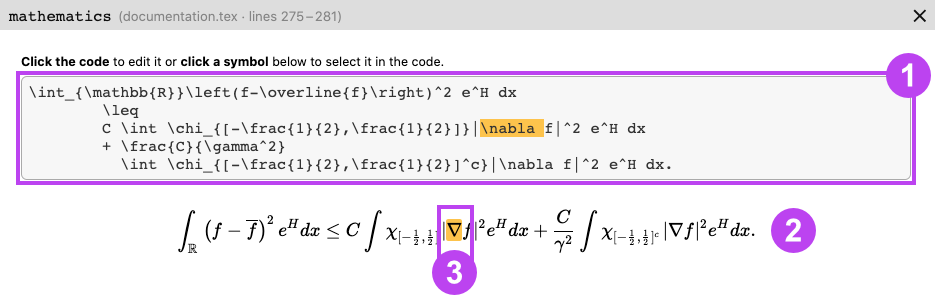
\includegraphics[width = \textwidth]{img/iir-imaths.png}
    \caption{The IIR of \texttt{imaths} environments. \figstep{1} The editable code of the formula. You can click it to \textbf{modify the code}, and the typeset formula will be \textbf{updated in real time}. \figstep{2} A typeset formula representing the code displayed above. \figstep{3} You can \textbf{point} and \textbf{click} most symbols in the typeset formula to respectively \textbf{highlight} or \textbf{select the piece of code} that generated it.}
    \label{fig:iir-imaths}
\end{figure}

An IIR for mathematics can be created with the \texttt{imaths} environment (\autoref{fig:iir-imaths}):

\begin{lstlisting}[style=custom-latex]
\begin{imaths}
    x = \alpha x + \beta y + \gamma
\end{imaths}
\end{lstlisting}

It behaves like the \texttt{align*} environment provided by the \texttt{amsmath} package: you can use all the commands accepted by \LaTeX{} in math mode inside, and you can align several formulae by using \verb|&| to align symbols vertically and \verb|\\| to break lines.

% This IIR enables you to edit the code of the formula (\figstep{1}) and \textbf{see the change in the typeset formula in real time} (\figstep{2}), as well as to \textbf{find} (by pointing) and to \textbf{select} (by clicking) the piece of code related to almost every symbol of the typeset formula (\figstep{3}).

\begin{info}
    When you edit the code of the formula in the IIR, the actual code of your \LaTeX{} document will \textbf{not} be updated until you click outside of the text area or press Enter.
\end{info}

\begin{warning}
    Some uncommon commands or environments may not be supported (it will compile, but the IIR will not work).
    User-defined commands are not supported either, unless the commands are defined \emph{within} the \texttt{imaths} environment.
\end{warning}

\begin{example}[nobreak]
    Writing

    \begin{lstlisting}[style=custom-latex-example]
\begin{imaths}
    \int_{\mathbb{R}}\left(f-\overline{f}\right)^2 e^H dx
    \leq
    C \int \chi_{[-\frac{1}{2},\frac{1}{2}]}|\nabla f|^2 e^H dx
    + \frac{C}{\gamma^2}
      \int \chi_{[-\frac{1}{2},\frac{1}{2}]^c}|\nabla f|^2 e^H dx.
\end{imaths}
    \end{lstlisting}
    
    will produce

    \begin{imaths}
        \int_{\mathbb{R}}\left(f-\overline{f}\right)^2 e^H dx
        \leq
        C \int \chi_{[-\frac{1}{2},\frac{1}{2}]}|\nabla f|^2 e^H dx
        + \frac{C}{\gamma^2}
          \int \chi_{[-\frac{1}{2},\frac{1}{2}]^c}|\nabla f|^2 e^H dx.
    \end{imaths}
\end{example}


%%%%%%%%%%%%%%%%%%%%%%%%%%%%%%%%%%%%%%%%%%%%%%%%%%%%%%%%%%%%%% IINCLUDEGRAPHICS


\newpage
\subsection{Images}

\begin{figure}[h!]
    \centering
    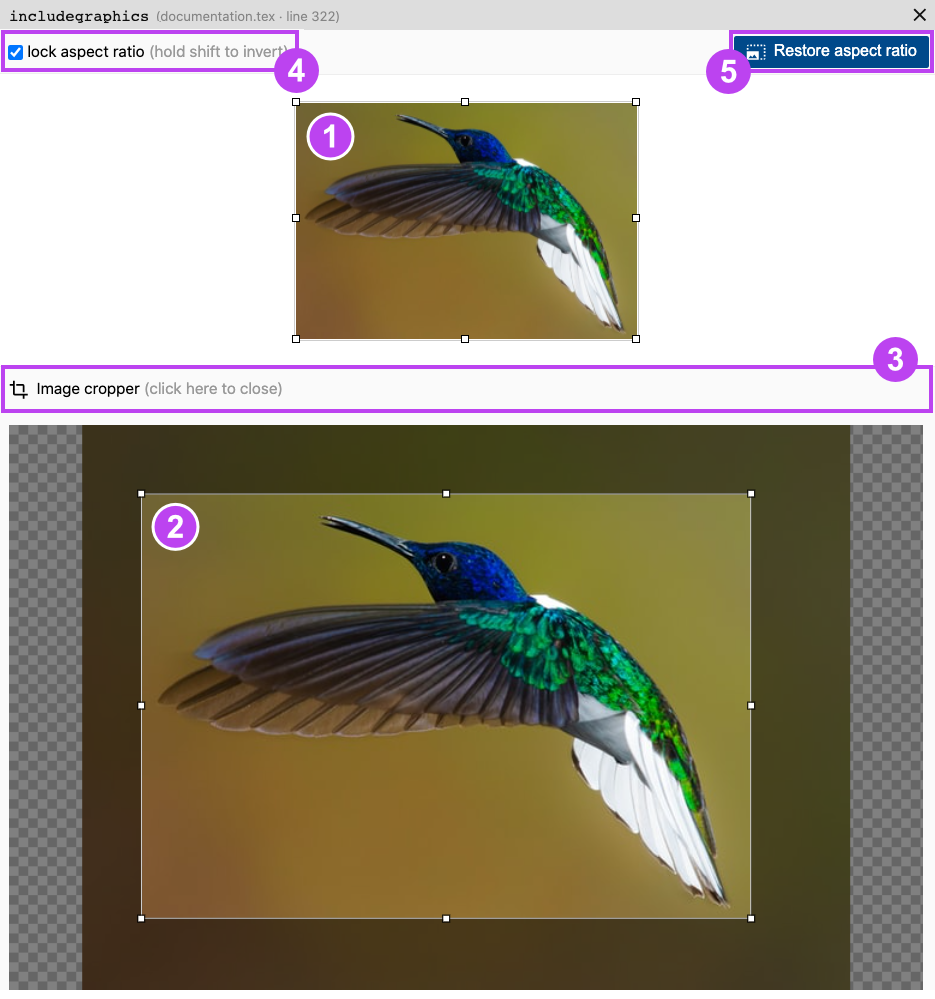
\includegraphics[width = .6\textwidth]{img/iir-iincludegraphics.png}
    \caption{The IIR of \texttt{iincludegraphics} commands. \figstep{1} The expected output of the command. You can \textbf{resize it} by dragging one of the handles around the image. \figstep{2} The area of the image to display. You can \textbf{move it} by dragging it and \textbf{resize it} by dragging one of the handles around the visible area. \figstep{3} You can display or hide the image cropper by clicking this bar. \figstep{4} You can hold the Shift key or uncheck this box to resize the image with a \textbf{non-natural aspect ratio}. If the image has a non-natural aspect ratio when the IIR is opened, the box will be unchecked by default. \figstep{5} You can resize the image to \textbf{restore its natural aspect ratio} by clicking this button.}
    \label{fig:iir-iincludegraphics}
\end{figure}

An IIR for images can be created with the \verb|\|\underline{\texttt{ii}}\verb|ncludegraphics| command, with two \texttt{i}s (\autoref{fig:iir-iincludegraphics}):

\begin{lstlisting}[style=custom-latex]
\iincludegraphics[width=\textwidth]{path/to/your/image.png}
\end{lstlisting}

It behaves like the \verb|\includegraphics| command provided by the \texttt{graphicx} package.
Only the \texttt{width}, \texttt{height}, \texttt{trim} and \texttt{clip} options are recognised by \iLaTeX{}.
You can still use all the other options supported by \verb|\includegraphics|, but they will be ignored and may be deleted by the IIR when you interact with it (as it can modify the code).

% This IIR enables you to \textbf{resize} (\figstep{1}) and to \textbf{crop} (\figstep{2} and \figstep{3}) the image (\ie only display a certain region of the image).
% To resize the image or the area to display, click and drag one of the handles displayed around the corresponding rectangular frame.
% It also enables you to lock/unlock the aspect ratio of the image or to restore the natural ratio (\figstep{5}). 

\begin{info}
    \iLaTeX{} supports the most common \emph{length macros} like \verb|\textwidth|, so you can freely use them in the options of a command like this one.
    It also supports relative length units (\texttt{em} and \texttt{ex}).
\end{info}

\begin{warning}
    PDF images are not supported (it will compile, but the IIR will not work correctly).
\end{warning}

\begin{example}
    Writing

    \begin{lstlisting}[style=custom-latex-example]
\iincludegraphics[width = 0.5\textwidth]{img/bird.jpg}
    \end{lstlisting}
    
    will produce

    \centering
    \iincludegraphics[width = 0.5\textwidth]{img/bird.jpg}
\end{example}


%%%%%%%%%%%%%%%%%%%%%%%%%%%%%%%%%%%%%%%%%%%%%%%%%%%%%%%%%%%%%% ITABULAR


\newpage
\subsection{Tables}

\begin{figure}[hb!]
    \centering
    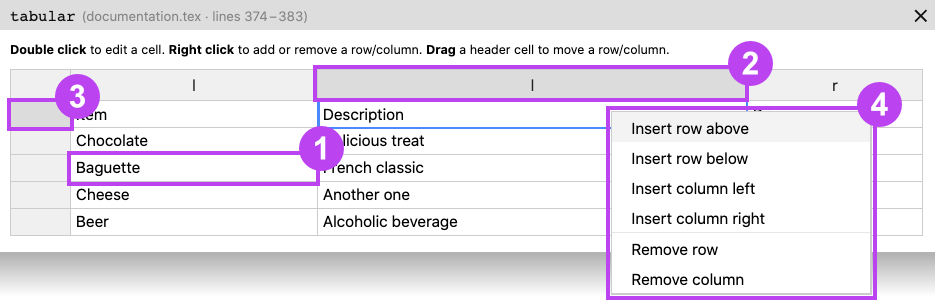
\includegraphics[width = \textwidth]{img/iir-itabular.png}
    \caption{The IIR of \texttt{itabular} environments. \figstep{1} A cell of the table. You can \textbf{edit} its content by double-clicking on it. \figstep{2} The header cell of a column. If \iLaTeX{} was able to parse the type of this column (\eg \texttt{l}, \texttt{c}, \texttt{r}), this cell contains it. You can \textbf{drag it} to \textbf{move the column}. \figstep{3} The header cell of a row. You can \textbf{drag it} to \textbf{move the row}. \figstep{4} You can display a \textbf{contextual menu} by right-clicking any cell of the table. It enables you to \textbf{insert} and \textbf{delete} \textbf{rows and columns}.}
    \label{fig:iir-itabular}
\end{figure}

An IIR for tables can be created with the \texttt{itabular} environment (\autoref{fig:iir-itabular}):

\begin{lstlisting}[style=custom-latex]
\begin{itabular}{llr}
    Item      & Description & Price \\
    Chocolate & ...         & 2.20  \\
    Baguette  & ...         & 0.90
\end{itabular}
\end{lstlisting}

It behaves like the \texttt{tabular} environment, and expects a mandatory argument (the list of column types).

% This IIR enables you to \textbf{edit any cell} by double-clicking on it (\figstep{1}), to \textbf{move} rows and columns by drag and dropping the header cell of the row/column (\figstep{2} and \figstep{3}), and to \textbf{insert and delete} rows and columns via a contextual menu displayed on right click (\figstep{4}).

\begin{info}
    Common formatting commands for tables such as \verb|\hline|, \verb|\toprule|, \verb|\midrule| and \verb|\bottomrule| are not considered as ``cell content'' by this IIR. You can safely use them, and \iLaTeX{} will do its best to ignore them and leave them in place.
\end{info}

\begin{warning}
    This IIR expects every line to contain the same number of cells, and is likely to dysfunction if it is not the case.
    In particular, that means that merged cells are not supported (it will compile, but the IIR will not work correctly).
\end{warning}

\begin{example}[nobreak]
    Writing

    \begin{lstlisting}[style=custom-latex-example]
\begin{itabular}{llr}
    \toprule
    Item  & Description & Price \\
    \midrule
    Chocolate & Delicious treat & 2.20  \\
    Baguette & French classic & 0.90  \\
    Cheese & Another one & 3.00  \\
    Beer & Alcoholic beverage & 4.50  \\
    \bottomrule
\end{itabular}
    \end{lstlisting}
    
    will produce

    \centering
    \begin{itabular}{llr}
        \toprule
        Item  & Description & Price \\
        \midrule
        Chocolate & Delicious treat & 2.20  \\
        Baguette & French classic & 0.90  \\
        Cheese & Another one & 3.00  \\
        Beer & Alcoholic beverage & 4.50  \\
        \bottomrule
    \end{itabular}
\end{example}


%%%%%%%%%%%%%%%%%%%%%%%%%%%%%%%%%%%%%%%%%%%%%%%%%%%%%%%%%%%%%% GRIDLAYOUT


\newpage
\subsection{Grid layouts}

\begin{figure}[h!]
    \centering
    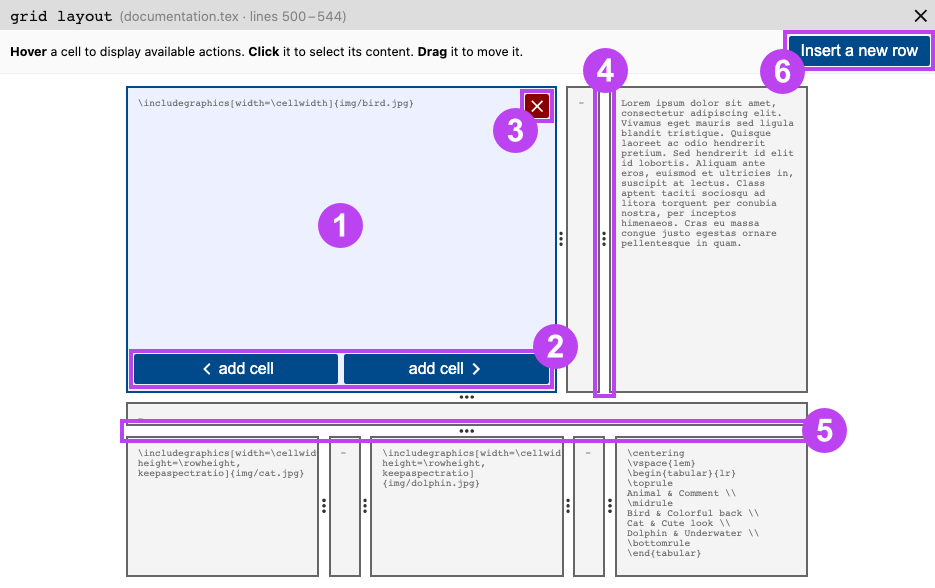
\includegraphics[width = .95\textwidth]{img/iir-gridlayout.png}
    \caption{The IIR of \texttt{gridlayout} environments. \figstep{1} A cell of the layout that is pointed by the mouse. It can be dragged to be moved before or after another cell. \figstep{2} Buttons to insert a new cell. \figstep{3} Button to remove the cell. \figstep{4} Separator between two cells. It can be dragged to resize the adjacent cells. \figstep{5} Separator between two rows. It can be dragged to resize the adjacent rows. \figstep{6} Button to insert a new row at the bottom of the grid.}
    \label{fig:iir-gridlayout}
\end{figure}

An IIR for grid layouts can be created with the \texttt{gridlayout} environment (\autoref{fig:iir-gridlayout}):

\begin{lstlisting}[style=custom-latex]
% This grid is as wide as the text (\textwidth) and 8cm tall
\begin{gridlayout}{\textwidth}{8cm}
    \begin{row}{0.6}
        \begin{cell}{1}
            % A cell as wide as the row that contains it
        \end{cell}
    \end{row}
    \begin{row}{0.4}
        \begin{cell}{0.33}
            % Bottom-left cell taking 1/3 of the row
        \end{cell}
        \begin{cell}{0.67}
            % Bottom-right cell taking 2/3 of the row
        \end{cell}
    \end{row}
\end{gridlayout}
\end{lstlisting}


Contrary to the other IIRs, this IIR is not a wrapper around an existing command or environment, but an \textbf{experimental structure} built to explore how an editor such as \iLaTeX{} could make it easier to manipulate this type of layout in \LaTeX{}.
Internally, it is built with a number of \texttt{minipage}s.
Every grid can contain rows (\texttt{row} environments), and every row can contain cells (\texttt{cell} environments).
A cell can contain \textbf{arbitrary content} (text, image, table, etc), but it \textbf{cannot contain other special commands or environments} such as \verb|\iincludegraphics|.

The \texttt{grid} environment expects two mandatory arguments: the \textbf{width} and the \textbf{height} of the grid.
The \texttt{row} and \texttt{cell} environments expect one mandatory argument each: the \textbf{relative height} of the row and the \textbf{relative width} of the cell.
These relative dimensions are \textbf{unitless numbers between 0 and 1} that must sum to 1 over all the cells of a row and over all the rows of the grid.
If they do not sum to 1, the document will compile, but the cells and the rows may not be positioned correctly, and the IIR 

% This IIR enables to manipulate the cells and the rows of the grid.
% Hovering a cell with your cursor (\figstep{1}) will display buttons to \textbf{insert a new cell} (\figstep{2}) and to \textbf{delete the cell} (\figstep{3}).
% It also enables to \textbf{move the cell} before or after another cell by drag and dropping it to the desired location.
% You can also \textbf{resize cells and rows} by dragging the separator between two of them (\figstep{4} and \figstep{5}).
% Finally, you can \textbf{insert a new row} (with a single cell) at the bottom of the grid by clicking the button in the top-right hand corner (\figstep{6}).

\begin{info}
    In every cell, you can use \verb|\cellwidth| and \verb|\rowheight|, two custom length macros relative to the current size of the cell that you can freely use (\eg to make an image have the same width or height than the cell).
\end{info}

\begin{warning}
    You should always use \textbf{at least one row} with \textbf{at least one cell} in a \texttt{gridlayout} environment, and you should avoid putting anything outside of a \texttt{cell} environment.
    Otherwise, you are likely to ``break'' the layout, and the IIR will not represent it correctly anymore.
\end{warning}

\begin{warning}
    \textbf{Empty cells}, such as cells acting as white space, appear to be ignored when the \texttt{cell} environments contain no symbol.
    You can fix this issue by putting a white space character in the body of the environment, such as a non-breaking space (\verb|~|).
\end{warning}

\begin{example}
    Writing

    \begin{lstlisting}[style=custom-latex-example]
\begin{gridlayout}{\textwidth}{11cm}
    \begin{row}{0.65}
        \begin{cell}{0.65}
            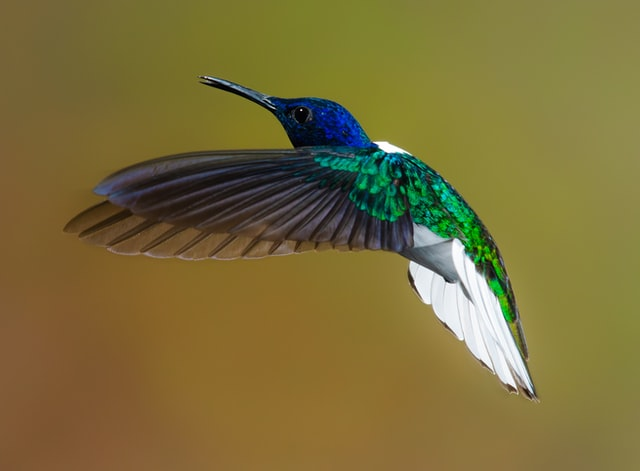
\includegraphics[width=\cellwidth]{img/bird.jpg}
        \end{cell}
        \begin{cell}{0.05}
            ~ % Separator
        \end{cell}
        \begin{cell}{0.3}
            Lorem ipsum dolor sit amet [...] in quam.
        \end{cell}
    \end{row}
    \begin{row}{0.05}
        \begin{cell}{1}
            ~ % Separator
        \end{cell}
    \end{row}
    \begin{row}{0.3}
        \begin{cell}{0.3}
            
\includegraphics[
                width=\cellwidth,
                height=\rowheight,
                keepaspectratio
            ]{img/cat.jpg}
        \end{cell}
        \begin{cell}{0.05}
            ~ % Separator
        \end{cell}
        \begin{cell}{0.3}
            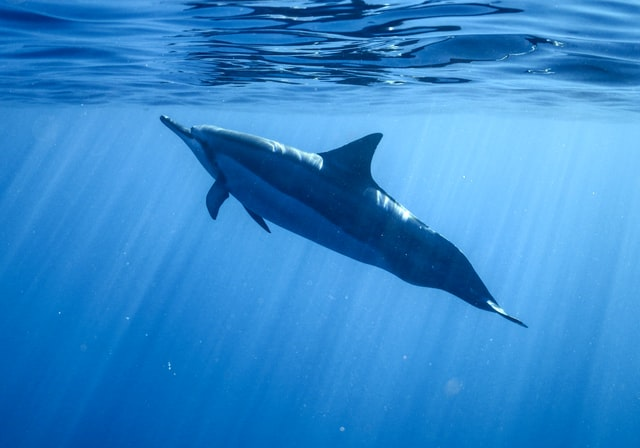
\includegraphics[
                width=\cellwidth,
                height=\rowheight,
                keepaspectratio
            ]{img/dolphin.jpg}
        \end{cell}
        \begin{cell}{0.05}
            ~ % Separator
        \end{cell}
        \begin{cell}{0.3}
            \centering
            \vspace{1em}
            \begin{tabular}{lr}
                \toprule
                Animal & Comment \\
                \midrule
                Bird & Colourful back \\
                Cat & Cute look \\
                Dolphin & Underwater \\
                \bottomrule
            \end{tabular}
        \end{cell}
    \end{row}
\end{gridlayout}
    \end{lstlisting}
    
    will produce (scaled to fit here)
    
    \centering
    \scalebox{0.8}{
    \begin{gridlayout}{\textwidth}{11cm}
        \begin{row}{0.65}
            \begin{cell}{0.65}
                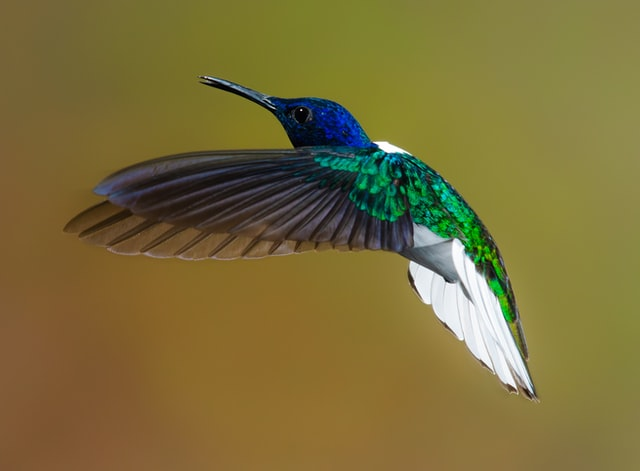
\includegraphics[width=\cellwidth]{img/bird.jpg}
            \end{cell}
            \begin{cell}{0.05}
                ~
            \end{cell}
            \begin{cell}{0.3}
                Lorem ipsum dolor sit amet, consectetur adipiscing elit. Vivamus eget mauris sed ligula blandit tristique. Quisque laoreet ac odio hendrerit pretium. Sed hendrerit id elit id lobortis. Aliquam ante eros, euismod et ultricies in, suscipit at lectus. Class aptent taciti sociosqu ad litora torquent per conubia nostra, per inceptos himenaeos. Cras eu massa congue justo egestas ornare pellentesque in quam.
            \end{cell}
        \end{row}
        \begin{row}{0.05}
            \begin{cell}{1}
                ~ 
            \end{cell}
        \end{row}
        \begin{row}{0.3}
            \begin{cell}{0.3}
                
\includegraphics[width=\cellwidth, height=\rowheight, keepaspectratio]{img/cat.jpg}
            \end{cell}
            \begin{cell}{0.05}
                ~
            \end{cell}
            \begin{cell}{0.3}
                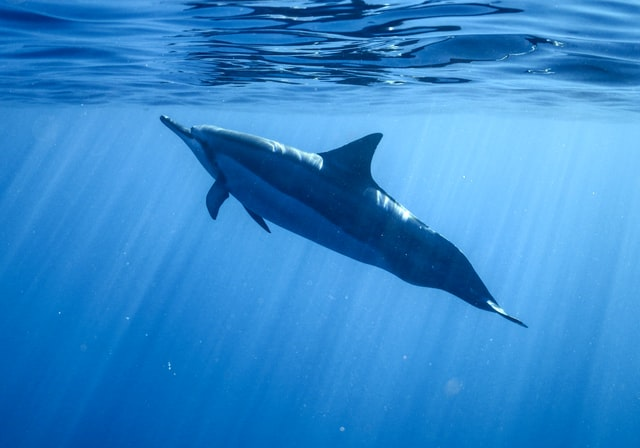
\includegraphics[width=\cellwidth, height=\rowheight, keepaspectratio]{img/dolphin.jpg}
            \end{cell}
            \begin{cell}{0.05}
                ~
            \end{cell}
            \begin{cell}{0.3}
                \centering
                \vspace{1em}
                \begin{tabular}{lr}
                    \toprule
                    Animal & Comment \\
                    \midrule
                    Bird & Colourful back \\
                    Cat & Cute look \\
                    Dolphin & Underwater \\
                    \bottomrule
                \end{tabular}
            \end{cell}
        \end{row}
    \end{gridlayout}
    }
\end{example}